\documentclass{article}

\usepackage[T1]{fontenc}    %Schriftart des Dokumentes
\usepackage[ngerman]{babel} %Dokumentensprache, hier Deutsch
\usepackage{amsmath, amssymb, stmaryrd} %mathematische Schriftzeichen
\usepackage{graphicx} %Einfügen von Grafiken
\usepackage{wrapfig}
\usepackage{bm}
\usepackage{afterpage}

\setlength{\parindent}{0pt} %Einrückung von Absätzen auf null gesetzt
\setlength{\parskip}{10pt} %Abstand zischen Absätzen auf 10pt gesetzt

\title{Versuch 35: Fotoeffekt}
\author{Matthias Kuntz}
\date{12.09.2023}

\begin{document}

\maketitle

%-------------------------EINLEITUNG-------------------------
\section{Einleitung}

In diesem Versuch soll mithilfe des Fotoeffekts das Planck'sche Wirkungsquantum $h$ bestimmt werden. Dazu wird der Fotostrom einer Fotozelle gemessen, die über einen Doppelprismaaufbau von einer Quecksilberlampe beleuchtet wird. Dabei wird das Licht der Lampe über die beiden Prismas in die verschiedenen Bestandteile aufgebrochen, von denen fünf nacheinander über einen beweglichen Spiegel auf die Fotozelle fixiert werden. Gemessen werden die Fotoströme mit der Gegenfeldmethode und es werden die Grenzenergien der beim Fotoeffekt emittierten Elektronen bestimmt, woraus dann das Plank'sche Wirkungsquantum bestimmt werden kann.  

\subsection{Physikalische Grundlagen}

Zu Beginn soll der Fotoeffekt erläutert werden, der auf der Grundlage basiert, dass Metalle sich bei ihrer Bildung aufteilen lassen in zum einen ein Metallgitter bestehend aus positiv geladenen Atomrümpfen und zum anderen delokalisierte Elektronen, welche sich praktisch frei im Metall bewegen können und als Leitungselektronen bezeichnet werden. Diese Elektronen können sich zwar im Metall frei bewegen, dieses aber nicht ohne die nötige Energie verlassen. Wie die Energie der Leitungselektronen verteilt ist, lässt sich aus der Temperaturabhängigen Fermiverteilung ablesen, zu sehen in Abbildung 1 links. Sie beschreibt die Wahrscheinlichkeit $W(E)$, dass ein Elektron im Metall die Energie $E$ hat. Wie man sehen kann, sind bei einer Temperatur von 0K alle Energiezustände bis zur sogenannten Fermikante $E_F$ gleichwahrscheinlich. Ist die Temperatur höher, so wird diese Kante aufgeweicht. 

Die Fermikante beschreibt hierbei die Energiegrenze, bis zu der alle Energiezustände von Leitungselektronen in einem Metall besetzt sind. Möchte man nun, dass ein Elektron mit der Energie $E_e$ das Metall verlässt, so muss dieses zunächst auf das Energieniveau der Fermikante $E_F$ gebracht und anschließend noch um eine zusätzliche Austrittsarbeit $A$ sowie um eine Energie $E_{Kin}$ erhöht werden, um das Metall mit der kinetischen Energie $E_{Kin}$ zu verlassen. 

Beim Fotoeffekt wird Metall mit Photonen bestrahlt, ergo mit Licht beleuchtet, und die Photonen geben den Leitungselektronen durch Zusammenstöße ihre Energie $h \nu$, gegeben über das Plank'sche Wirkungsquantum $h$ und die Frequenz $\nu$. Ist diese Energie ausreichend groß, so kann das Elektron das Metall verlassen. Das gesamte Konzept ist auch in Abbildung 1 rechts dargestellt.

\begin{figure} [!ht]
    \centering
    \includegraphics[width=10cm]{graphics/abb1.jpg}
    \caption{Fermiverteilung (links) \& Potenzialtopfmodell (rechts)}
\end{figure}

Aus dem Energiesatz folgt dann:

\begin{equation}
    h \nu = A + (E_F - E_e) + E_{Kin}
\end{equation}

Dabei wird die kinetische Energie maximiert, wenn die Elektronen bereits an der Fermikante sind, wodurch gilt:

\begin{equation}
    E_{Kin_{max}} = h \nu - A
\end{equation}

Der Aufbau einer Fotozelle, wie sie in diesem Versuch verwendet wird, ist in Abbildung 2 links skizziert. Zwischen Kathode und Anode lässt sich eine variable Spannung anlegen, die bestimmt, welche Elektronen noch die Anode erreichen. Bei höherer negativer Spannung erreichen nur noch Elektronen mit hoher kinetischer Energie die Fotozelle, wird sie zu hoch werden alle Elektronen vorher abgelenkt. Für positive Spannungen bleibt der gemessene Fotostrom konstant. Ähnlich wie bei der Fermiverteilung ist die Strom-Spannungskennlinie einer Fotozelle temperaturabhängig und verweicht die Kanten bei Temperaturen größer als 0K, was in Abbildung 2 rechts zu erkennen ist. 

\begin{figure} [!ht]
    \centering
    \includegraphics[width=10cm]{graphics/abb2.jpg}
    \caption{Skizze einer Fotozelle (links) \& Strom-Spannungskennlinie einer realen Fotozelle (rechts)}
\end{figure}

\newpage

Zur Bestimmung der Spannung $U_S$, bei der der Fotostrom im Falle einer idealen Fotozelle bei T$=$0K verschwinden würde, sind Angaben abhängig von der Fotozelle nötig. Für die in diesem Versuch verwendete Fotozelle ergibt sich $I \propto U^2$ und somit die Sperrspannung $U_S$ als:

\begin{equation}
    e U_S = E_{Kin_{max}} = h \nu - A \propto \sqrt{I}
\end{equation}

Wobei $e$ die Elementarladung ist.

\newpage

\subsection{Versuchsaufbau}

Der Versuchsaufbau ist in Abbildung 3 skizziert. Das Licht der Hg-Lampe wird zunächst über einen Kollimator auf das Doppelprisma geleitet, wo es aufgeteilt wird und auf einen beweglichen Spiegel trifft, der das Licht in das Fernrohr weiterleitet, in dem sich die Fotozelle befindet. Mit einem Hebel lässt sich ein Spiegel im Fernrohr hochklappen, der das einfallende Licht auf einen Schirm ableitet, auf dem die Spektrallinien beobachtet und mithilfe des beweglichen Spiegels so verschoben werden können, dass immer nur eine Linie auf die Fotozelle geworfen wird. Treffen Photonen auf die Fotokathode, so lösen sich Elektronen mit der kinetischen Energie $E_{Kin_{max}} = h \nu - A$ aus dieser heraus. Ist nun der Anodenring über Kabel mit der Kathode verbunden, so fließt ein Strom. Die Kathode wird geerdet und der Anode eine Vorspannung gegeben.

\begin{figure} [!ht]
    \centering
    \includegraphics[width=10cm]{graphics/abb3.jpg}
    \caption{Skizze des Versuchsaufbaus}
\end{figure}

\newpage
%---------------VERSUCHSPROTOKOLL MIT MESSDATEN---------------
\newpage

\section{Versuchsprotokoll mit Messdaten}

\includegraphics[width=\textwidth]{graphics/mess1.jpg}
\newpage
\includegraphics[width=\textwidth]{graphics/mess2.jpg}
\newpage
\includegraphics[width=\textwidth]{graphics/mess3.jpg}
\newpage

\addtocounter{table}{5}

%-------------------------AUSWERTUNG-------------------------
\section{Auswertung}

\subsection{Bestimmung der Sperrspannungen}

Zunächst werden die Werte der Tabellen 1 bis 5 ausgewertet, indem folgendes berechnet wird: Der Fehler der gemessenen Spannungen $\Delta U_I$ wie im Messprotokoll angegeben, die Differenz aus gemessener Spannung und Untergrundspannung $U_I - U_{I0}$ mitsamt Fehler $\Delta (U_I - U_{I0})$ und die Wurzel aus der Differenz $\sqrt{U_I - U_{I0}}$ sowie ihr Fehler $\Delta \sqrt{U_I - U_{I0}}$. Die Fehler bestimmt man über das Fehlerfortpflangungsgesetz mit:

\begin{equation}
    \begin{split}
        \Delta (U_I - U_{I0}) &= \sqrt{(\Delta U_I)^2 + (\Delta U_{I0})^2}\\
        \Delta \sqrt{U_I - U_{I0}} &= \sqrt{\left( \frac{\Delta (U_I - U_{I0})}{2\sqrt{U_I - U_{I0}}} \right)^2}
    \end{split}
\end{equation}

Die Ergebnisse sind in den Tabellen 6 bis 10 dargestellt.

Anschließend werden die bestimmten Werte der Wurzeln in einem Diagramm auf der Ordiante und die eingestellten Vorspannungen auf der Abszisse eingezeichnet. Für jede bemessene Linie wird hierbei ein eigenes Diagramm angefertigt. Die Ergebnisse sind in Abbildungen 4 bis 8 zu sehen.

Aus diesen Diagrammen ließt man, indem man an den linearen Teil in der Mitte der Punkte eine Gerade anlegt und diese so weit verlängert, bis sie auf die Abszisse trifft, ergo bei $\sqrt{U_I - U_{I0}} = 0$, die Spannung $U_S$ ab. Den Fehler $\Delta U_S$ bestimmt man, indem man an den linearen Teil eine Fehlergerade anlegt und die Differenz zwischen dem Wert, bei dem die Fehlergerade die Abszisse trifft, und dem bereits bestimmten $U_S$ nimmt.

Die bestimmten Sperrspannungen $U_S$ werden ihren Wellenlängen $\lambda$ zugeordnet und man erhält:

\addtocounter{table}{5}

\begin{table}[h!]
    \centering
    \begin{tabular}{c|c}
    $\bm{\lambda}$ [nm] & $\bm{U_S}$ [V] \\ \hline
    365 & $-(1,93 \pm 0,02)$ \\
    405 & $-(1,66 \pm 0,02)$ \\
    435,8 & $-(1,43 \pm 0,05)$ \\
    546,1 & $-(0,84 \pm 0,03)$ \\
    578 & $-(0,61 \pm 0,03)$ \\
    \end{tabular}
    \caption{Spannungen $U_S$ mit den zugehörigen Wellenlängen $\lambda$}
\end{table}


\addtocounter{table}{-6}
%------Tabellen------
\afterpage{
    
\begin{table}[!ht]
    \centering
    \caption{Auswertung der UV-Linie}
    \resizebox{\textwidth}{!}{\begin{tabular}{c|c|c|c|c|c|c}
        $\bm{U}$ [V] & $\bm{U_I}$ [mV] & $\bm{\Delta U_I}$ [mV] & $\bm{U_I - U_{I0}}$ [mV] & $\bm{\Delta (U_I - U_{I0})}$ [mV] & $\bm{\sqrt{U_I - U_{I0}}}$ [$\sqrt{\text{mV}}$] & $\bm{\Delta \sqrt{U_I - U_{I0}}}$ [$\sqrt{\text{mV}}$] \\ \hline
        0,0 & 3419 & 8 & 3438 & 9 & 58,634 & 0,026 \\ 
        -0,1 & 3095 & 7 & 3114 & 9 & 55,803 & 0,027 \\ 
        -0,2 & 2818 & 7 & 2837 & 9 & 53,263 & 0,028 \\ 
        -0,3 & 2520 & 7 & 2539 & 9 & 50,388 & 0,029 \\ 
        -0,4 & 2224 & 7 & 2243 & 8 & 47,36 & 0,03 \\ 
        -0,5 & 1964 & 7 & 1983 & 8 & 44,53 & 0,03 \\ 
        -0,6 & 1705 & 6 & 1724 & 8 & 41,52 & 0,03 \\ 
        -0,7 & 1452 & 6 & 1471 & 8 & 38,35 & 0,04 \\ 
        -0,8 & 1230 & 6 & 1249 & 8 & 35,34 & 0,04 \\ 
        -0,9 & 1020 & 6 & 1039 & 8 & 32,23 & 0,04 \\ 
        -1,0 & 822 & 6 & 841 & 8 & 29,00 & 0,05 \\ 
        -1,1 & 653 & 6 & 672 & 7 & 25,92 & 0,05 \\ 
        -1,2 & 505 & 5 & 524 & 7 & 22,89 & 0,06 \\ 
        -1,3 & 364 & 5 & 383 & 7 & 19,57 & 0,07 \\ 
        -1,4 & 258 & 5 & 277 & 7 & 16,64 & 0,08 \\ 
        -1,5 & 175 & 5 & 194 & 7 & 13,93 & 0,10 \\ 
        -1,6 & 108 & 5 & 127 & 7 & 11,27 & 0,12 \\ 
        -1,7 & 53 & 5 & 72 & 7 & 8,49 & 0,16 \\ 
        -1,8 & 15 & 5 & 34 & 7 & 5,83 & 0,23 \\ 
        ~ & ~ & ~ & ~ & ~ & ~ & ~ \\
        $\bm{U}$ [V] & $\bm{U_{I0}}$ [mV] & $\bm{\Delta U_{I0}}$ [mV] & ~ & ~ & ~ & ~ \\ \hline
        ~ & ~ & ~ & ~ & ~ & ~ & ~ \\
        -4,0 & -19 & 5 & ~ & ~ & ~ & ~ \\ 
    \end{tabular}}
\end{table}

\begin{table}[!ht]
    \centering
    \caption{Auswertung der violetten Linie}
    \resizebox{\textwidth}{!}{\begin{tabular}{c|c|c|c|c|c|c}
        $\bm{U}$ [V] & $\bm{U_I}$ [mV] & $\bm{\Delta U_I}$ [mV] & $\bm{U_I - U_{I0}}$ [mV] & $\bm{\Delta (U_I - U_{I0})}$ [mV] & $\bm{\sqrt{U_I - U_{I0}}}$ [$\sqrt{\text{mV}}$] & $\bm{\Delta \sqrt{U_I - U_{I0}}}$ [$\sqrt{\text{mV}}$] \\ \hline
        0,3 & 4461 & 9 & 4477 & 10 & 66,910 & 0,024 \\ 
        0,2 & 4068 & 8 & 4084 & 10 & 63,906 & 0,024 \\ 
        0,1 & 3714 & 8 & 3730 & 9 & 61,074 & 0,025 \\ 
        0,0 & 3347 & 8 & 3363 & 9 & 57,991 & 0,026 \\ 
        -0,1 & 2987 & 7 & 3003 & 9 & 54,800 & 0,027 \\ 
        -0,2 & 2652 & 7 & 2668 & 9 & 51,653 & 0,029 \\ 
        -0,3 & 2313 & 7 & 2329 & 8 & 48,26 & 0,03 \\ 
        -0,4 & 2004 & 7 & 2020 & 8 & 44,94 & 0,03 \\ 
        -0,5 & 1706 & 6 & 1722 & 8 & 41,50 & 0,03 \\ 
        -0,6 & 1431 & 6 & 1447 & 8 & 38,04 & 0,04 \\ 
        -0,7 & 1187 & 6 & 1203 & 8 & 34,68 & 0,04 \\ 
        -0,8 & 943 & 6 & 959 & 8 & 30,97 & 0,04 \\ 
        -0,9 & 726 & 6 & 742 & 8 & 27,24 & 0,05 \\ 
        -1,0 & 552 & 5 & 568 & 7 & 23,83 & 0,06 \\ 
        -1,1 & 378 & 5 & 394 & 7 & 19,85 & 0,07 \\ 
        -1,2 & 250 & 5 & 266 & 7 & 16,31 & 0,08 \\ 
        -1,3 & 149 & 5 & 165 & 7 & 12,85 & 0,10 \\ 
        -1,4 & 71 & 5 & 87 & 7 & 9,33 & 0,14 \\ 
        -1,5 & 19 & 5 & 35 & 7 & 5,92 & 0,23 \\ 
        ~ & ~ & ~ & ~ & ~ & ~ & ~ \\ 
        $\bm{U}$ [V] & $\bm{U_{I0}}$ [mV] & $\bm{\Delta U_{I0}}$ [mV] & ~ & ~ & ~ & ~ \\ \hline
        ~ & ~ & ~ & ~ & ~ & ~ & ~ \\
        -4 & -16 & 5 \\ 
    \end{tabular}}
\end{table}

    \clearpage
}

\afterpage{

\begin{table}[!ht]
    \centering
    \caption{Auswertung der blauen Linie}
    \resizebox{\textwidth}{!}{\begin{tabular}{c|c|c|c|c|c|c}
        $\bm{U}$ [V] & $\bm{U_I}$ [mV] & $\bm{\Delta U_I}$ [mV] & $\bm{U_I - U_{I0}}$ [mV] & $\bm{\Delta (U_I - U_{I0})}$ [mV] & $\bm{\sqrt{U_I - U_{I0}}}$ [$\sqrt{\text{mV}}$] & $\bm{\Delta \sqrt{U_I - U_{I0}}}$ [$\sqrt{\text{mV}}$] \\ \hline
        0,3 & 5735 & 10 & 5759 & 11 & 75,888 & 0,022 \\ 
        0,2 & 5195 & 9 & 5219 & 10 & 72,243 & 0,022 \\ 
        0,1 & 4714 & 9 & 4738 & 10 & 68,833 & 0,023 \\ 
        0,0 & 4161 & 8 & 4185 & 10 & 64,692 & 0,024 \\ 
        -0,1 & 3700 & 8 & 3724 & 9 & 61,025 & 0,025 \\ 
        -0,2 & 3260 & 8 & 3284 & 9 & 57,306 & 0,026 \\ 
        -0,3 & 2796 & 7 & 2820 & 9 & 53,104 & 0,028 \\ 
        -0,4 & 2370 & 7 & 2394 & 9 & 48,929 & 0,030 \\ 
        -0,5 & 1968 & 7 & 1992 & 8 & 44,63 & 0,03 \\ 
        -0,6 & 1605 & 6 & 1629 & 8 & 40,36 & 0,04 \\ 
        -0,7 & 1282 & 6 & 1306 & 8 & 36,14 & 0,04 \\ 
        -0,8 & 977 & 6 & 1001 & 8 & 31,64 & 0,04 \\ 
        -0,9 & 686 & 6 & 710 & 7 & 26,65 & 0,05 \\ 
        -1,0 & 443 & 5 & 467 & 7 & 21,61 & 0,06 \\ 
        -1,1 & 255 & 5 & 279 & 7 & 16,70 & 0,08 \\ 
        -1,2 & 125 & 5 & 149 & 7 & 12,21 & 0,11 \\ 
        -1,3 & 33 & 5 & 57 & 7 & 7,55 & 0,18 \\ 
        ~ & ~ & ~ & ~ & ~ & ~ & ~ \\ 
        $\bm{U}$ [V] & $\bm{U_{I0}}$ [mV] & $\bm{\Delta U_{I0}}$ [mV] & ~ & ~ & ~ & ~ \\ \hline
        ~ & ~ & ~ & ~ & ~ & ~ & ~ \\
        -4,0 & -24 & 5 & ~ & ~ & ~ & ~\\ 
    \end{tabular}}
\end{table}

\begin{table}[!ht]
    \centering
    \caption{Auswertung der grünen Linie}
    \resizebox{\textwidth}{!}{\begin{tabular}{c|c|c|c|c|c|c}
        $\bm{U}$ [V] & $\bm{U_I}$ [mV] & $\bm{\Delta U_I}$ [mV] & $\bm{U_I - U_{I0}}$ [mV] & $\bm{\Delta (U_I - U_{I0})}$ [mV] & $\bm{\sqrt{U_I - U_{I0}}}$ [$\sqrt{\text{mV}}$] & $\bm{\Delta \sqrt{U_I - U_{I0}}}$ [$\sqrt{\text{mV}}$] \\ \hline
        0,3 & 4533 & 9 & 4545 & 10 & 67,417 & 0,023 \\ 
        0,2 & 3920 & 8 & 3932 & 10 & 62,706 & 0,025 \\ 
        0,1 & 3337 & 8 & 3349 & 9 & 57,871 & 0,026 \\ 
        0,0 & 2814 & 7 & 2826 & 9 & 53,160 & 0,028 \\ 
        -0,1 & 2213 & 7 & 2225 & 8 & 47,17 & 0,03 \\ 
        -0,2 & 1723 & 6 & 1735 & 8 & 41,65 & 0,03 \\ 
        -0,3 & 1263 & 6 & 1275 & 8 & 35,71 & 0,04 \\ 
        -0,4 & 850 & 6 & 862 & 8 & 29,36 & 0,05 \\ 
        -0,5 & 505 & 5 & 517 & 7 & 22,74 & 0,06 \\ 
        -0,6 & 253 & 5 & 265 & 7 & 16,28 & 0,08 \\ 
        -0,7 & 92 & 5 & 104 & 7 & 10,20 & 0,13 \\ 
        -0,8 & 17 & 5 & 29 & 7 & 5,39 & 0,25 \\ 
        ~ & ~ & ~ & ~ & ~ & ~ & ~ \\
        $\bm{U}$ [V] & $\bm{U_{I0}}$ [mV] & $\bm{\Delta U_{I0}}$ [mV] & ~ & ~ & ~ & ~ \\ \hline
        ~ & ~ & ~ & ~ & ~ & ~ & ~ \\
        -4 & -12 & 5 & ~ & ~ & ~ & ~ \\ 
    \end{tabular}}
\end{table}

\begin{table}[!ht]
    \centering
    \caption{Auswertung der gelben Linie}
    \resizebox{\textwidth}{!}{\begin{tabular}{c|c|c|c|c|c|c}
        $\bm{U}$ [V] & $\bm{U_I}$ [mV] & $\bm{\Delta U_I}$ [mV] & $\bm{U_I - U_{I0}}$ [mV] & $\bm{\Delta (U_I - U_{I0})}$ [mV] & $\bm{\sqrt{U_I - U_{I0}}}$ [$\sqrt{\text{mV}}$] & $\bm{\Delta \sqrt{U_I - U_{I0}}}$ [$\sqrt{\text{mV}}$] \\ \hline
        0,3 & 2355 & 7 & 2360 & 9 & 48,58 & 0,03 \\ 
        0,2 & 1919 & 7 & 1924 & 8 & 43,86 & 0,03 \\ 
        0,1 & 1531 & 6 & 1536 & 8 & 39,19 & 0,04 \\ 
        0,0 & 1156 & 6 & 1161 & 8 & 34,07 & 0,04 \\ 
        -0,1 & 800 & 6 & 805 & 8 & 28,37 & 0,05 \\ 
        -0,2 & 509 & 5 & 514 & 7 & 22,67 & 0,06 \\ 
        -0,3 & 297 & 5 & 302 & 7 & 17,38 & 0,08 \\ 
        -0,4 & 131 & 5 & 136 & 7 & 11,66 & 0,11 \\ 
        -0,5 & 54 & 5 & 59 & 7 & 7,68 & 0,17 \\ 
        -0,6 & 20 & 5 & 25 & 7 & 5,00 & 0,27 \\ 
        ~ & ~ & ~ & ~ & ~ & ~ & ~ \\
        $\bm{U}$ [V] & $\bm{U_{I0}}$ [mV] & $\bm{\Delta U_{I0}}$ [mV] & ~ & ~ & ~ & ~ \\ \hline
        ~ & ~ & ~ & ~ & ~ & ~ & ~ \\
        -4 & -5 & 5 & ~ & ~ & ~ & ~ \\ 
    \end{tabular}}
\end{table}

    \clearpage
}

%--------------------Diagramme---------------------

\afterpage{
\begin{figure} [p]
    \centering
    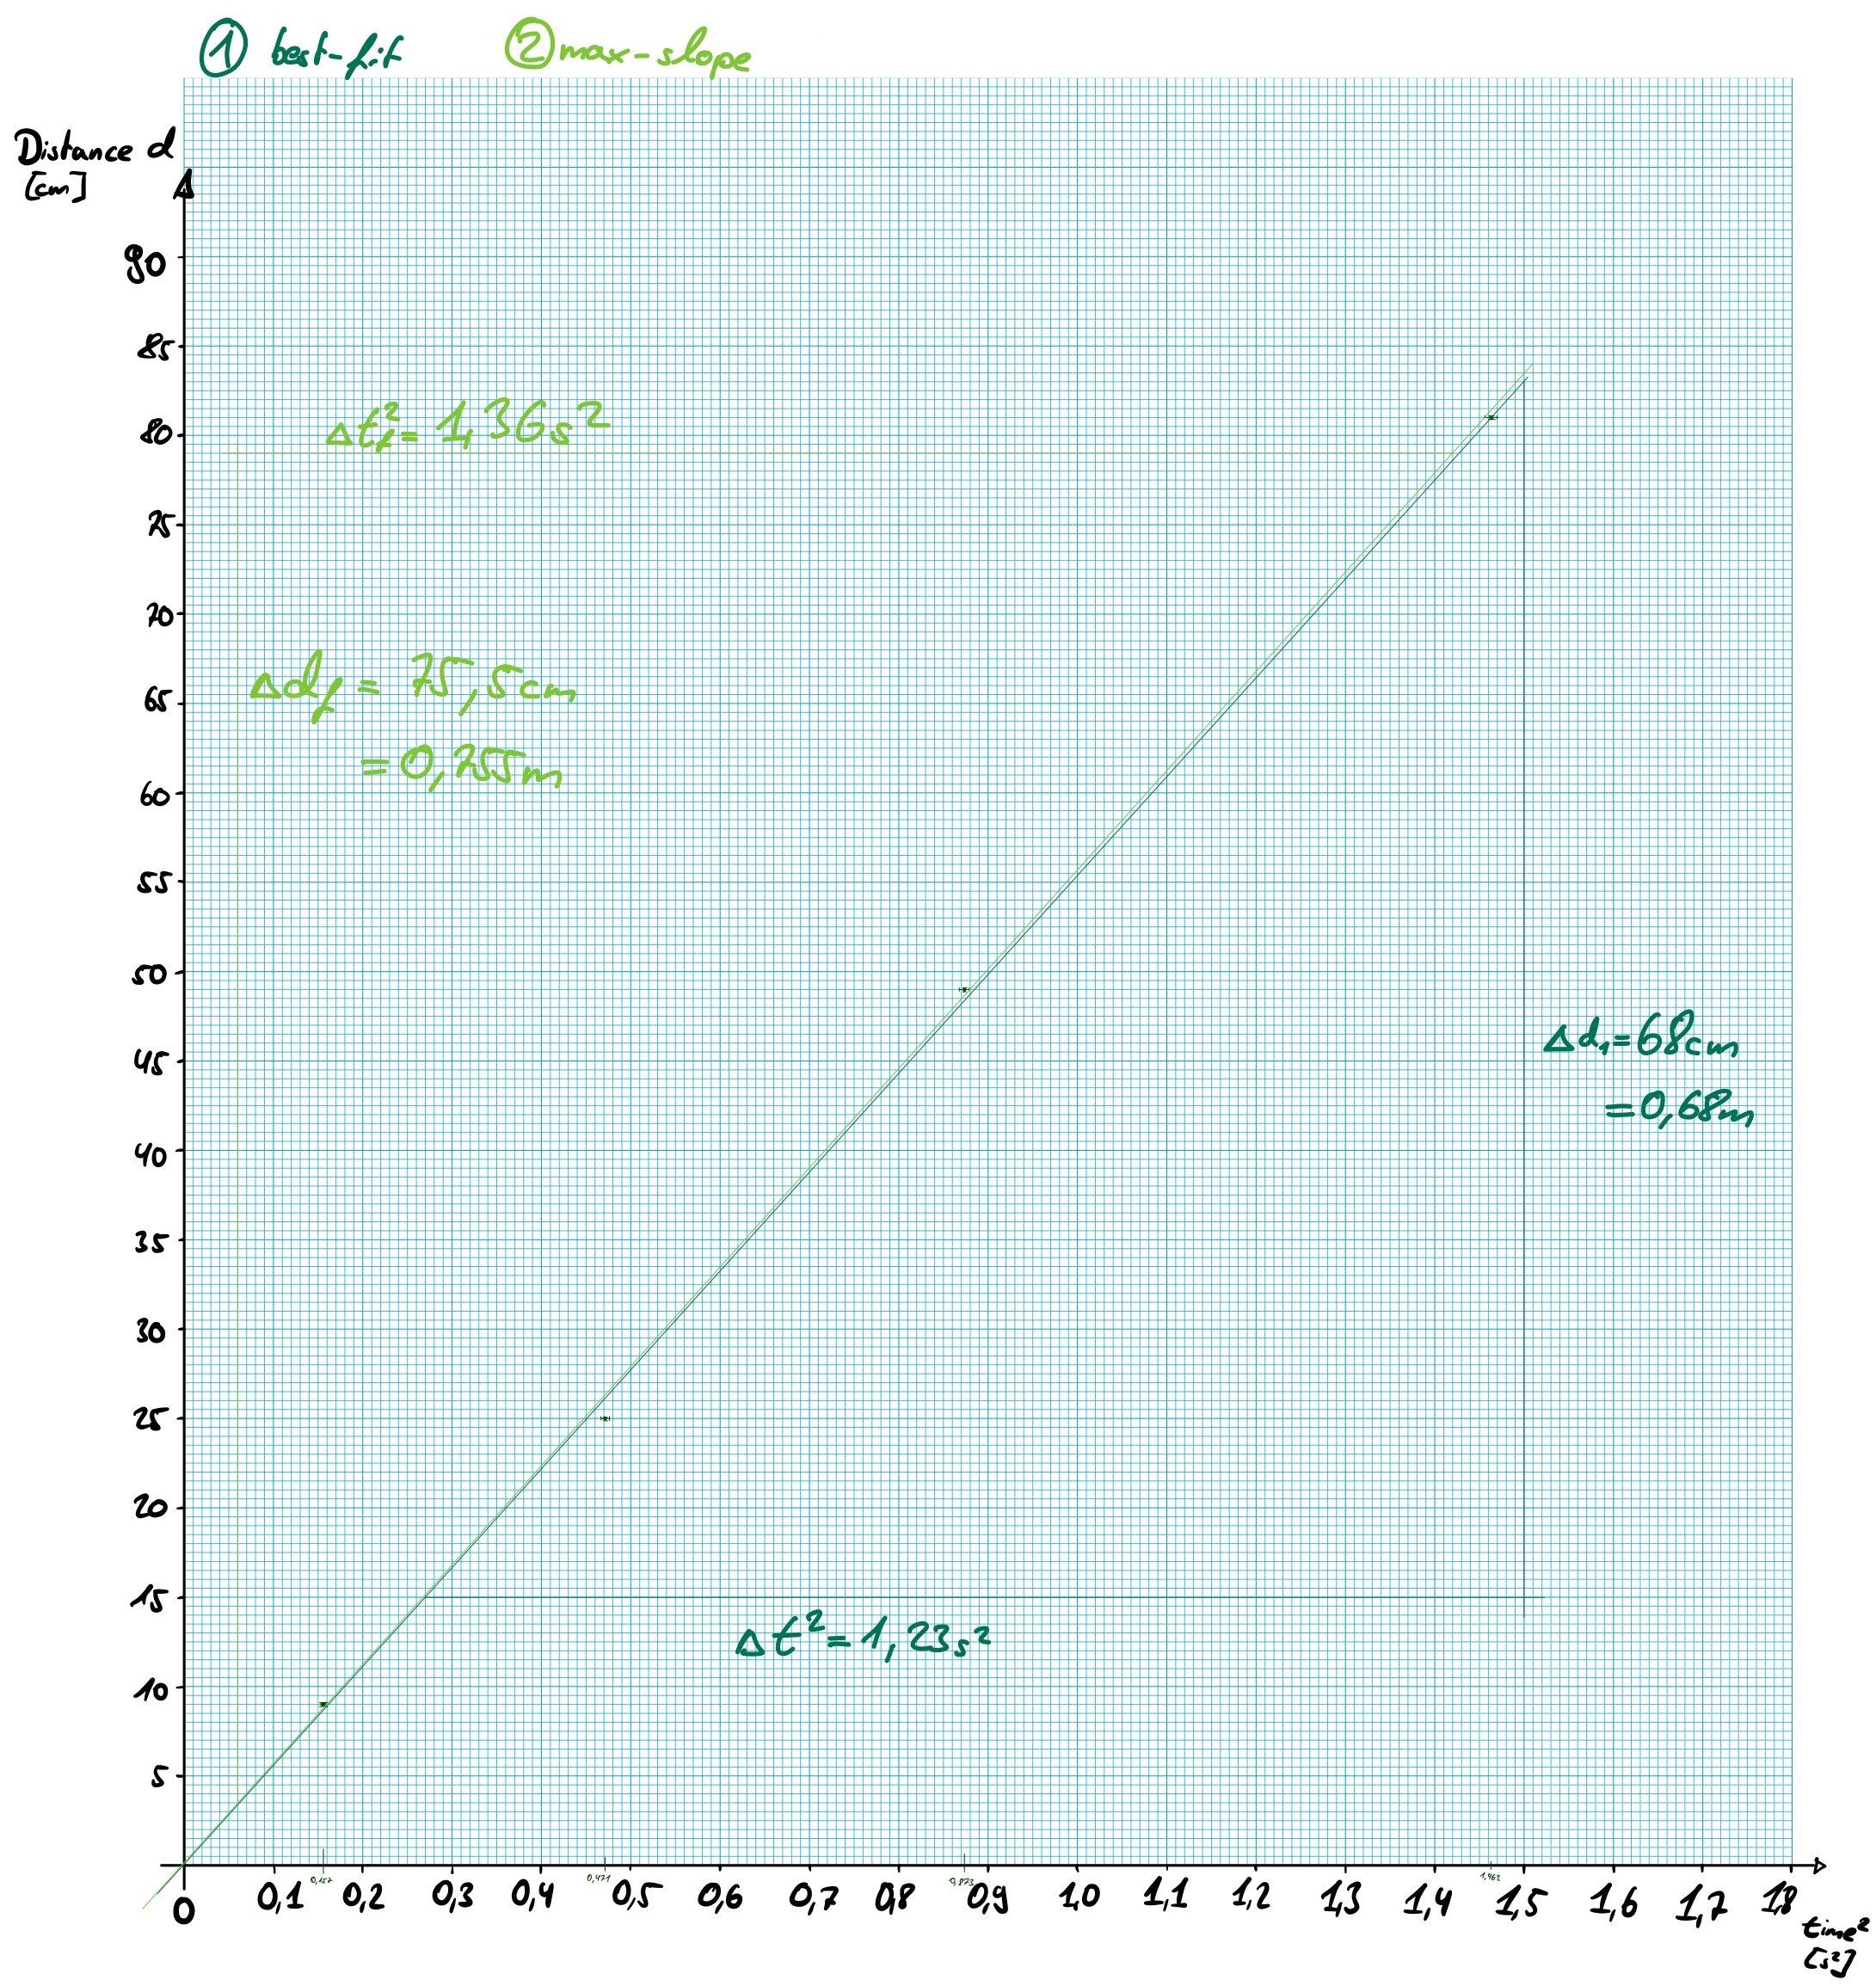
\includegraphics[width=\textwidth]{graphics/dia/dia1.pdf}
    \caption{Wurzel gegen Vorspannung: UV-Linie}
\end{figure}
\clearpage
}

\afterpage{
\begin{figure} [p]
    \centering
    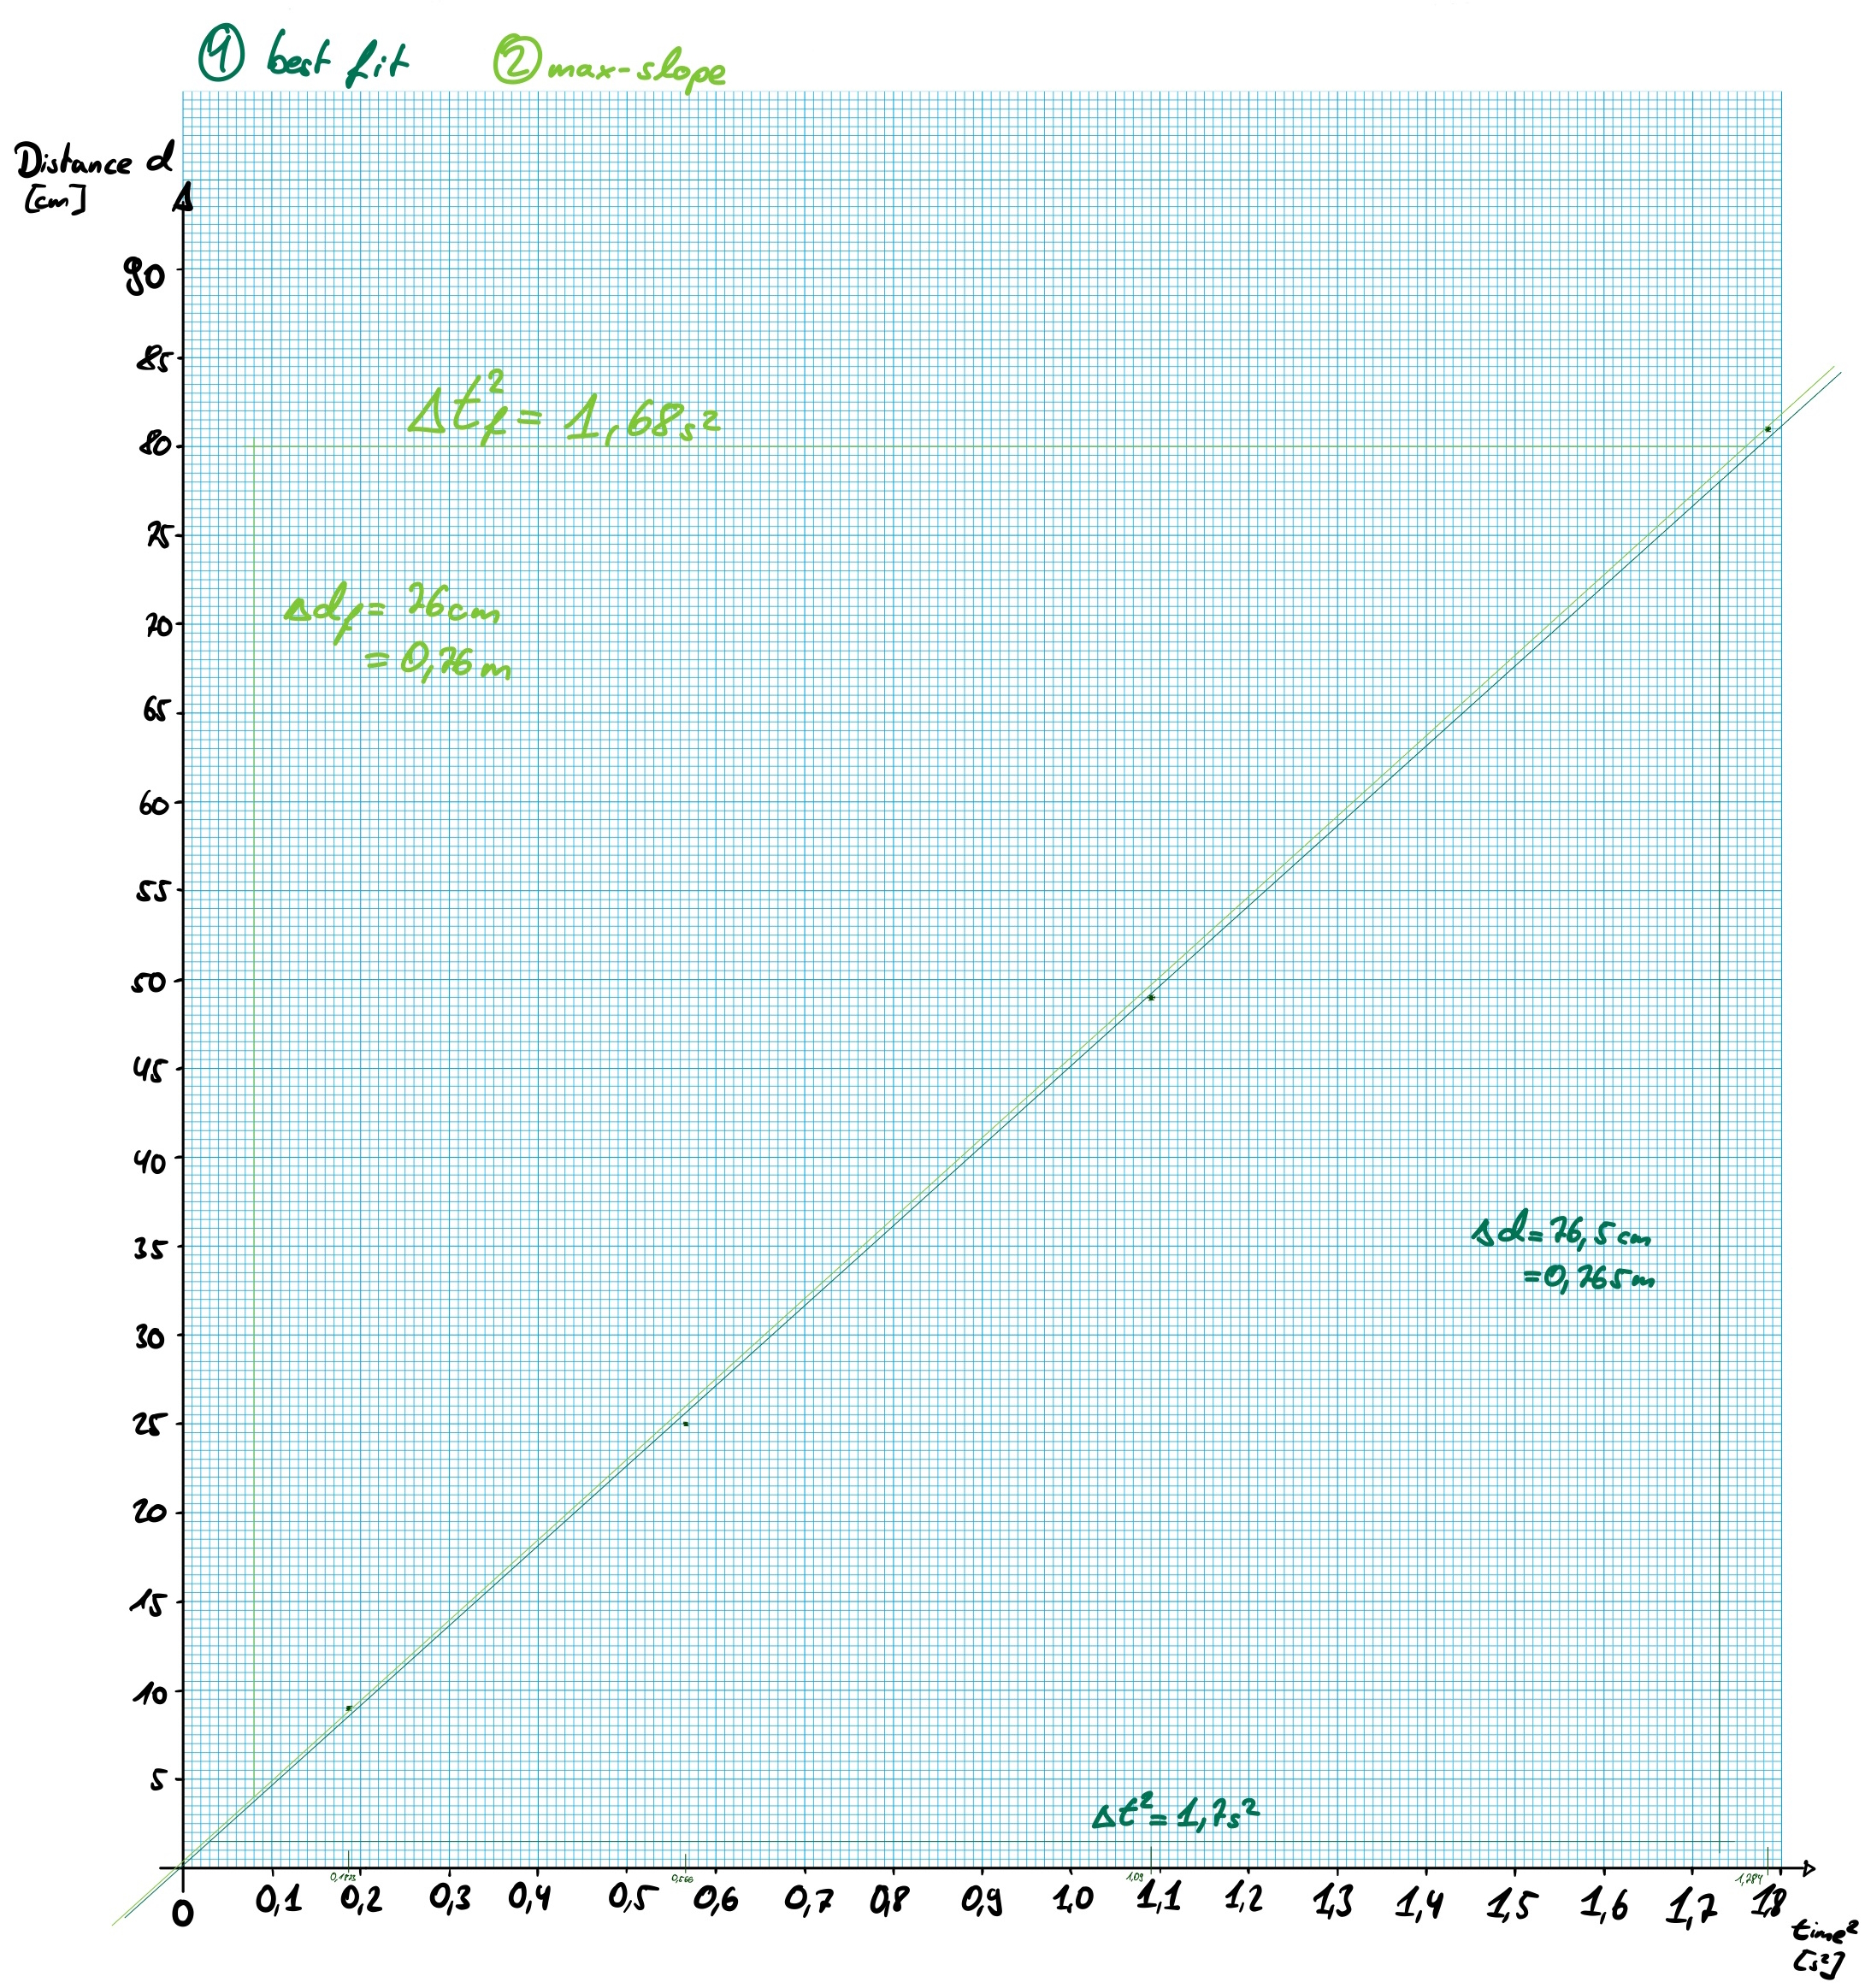
\includegraphics[width=\textwidth]{graphics/dia/dia2.pdf}
    \caption{Wurzel gegen Vorspannung: violette Linie}
\end{figure}
\clearpage
}

\afterpage{
\begin{figure} [p]
    \centering
    \includegraphics[width=\textwidth]{graphics/dia/dia3.pdf}
    \caption{Wurzel gegen Vorspannung: blaue Linie}
\end{figure}
\clearpage
}

\afterpage{
\begin{figure} [p]
    \centering
    \includegraphics[width=\textwidth]{graphics/dia/dia4.pdf}
    \caption{Wurzel gegen Vorspannung: grüne Linie}
\end{figure}
\clearpage
}

\afterpage{
\begin{figure} [p]
    \centering
    \includegraphics[width=\textwidth]{graphics/dia/dia5.pdf}
    \caption{Wurzel gegen Vorspannung: gelbe Linie}
\end{figure}
\clearpage
}

%--------------------------------------------------

\newpage

\subsection{Bestimmung des Plank'schen Wirkungsquantums $h$}

In einem weiteren Diagramm sollen die bestimmten Sperrspannungen der jeweiligen Linien gegen die Frequenz aufgetragen werden. 

Dazu werden zunächst die Frequenzen bestimmt mit $f=\frac{c}{\lambda}$, wobei $c=299 792 458 \frac{m}{s}$ (Wikipedia, Stand: 14.09.2023) die Lichtgeschwindigkeit ist:

\begin{table}[h!]
    \centering
    \begin{tabular}{c|c|c}
    $\bm{U_S}$ [V] & $\bm{\lambda}$ [nm] & $f$ [Hz] \\ \hline
    $-(1,93 \pm 0,02)$ & 365 &  8,21 $\cdot \ 10^{14}$ \\
    $-(1,66 \pm 0,02)$ & 405 & 7,40 $\cdot \ 10^{14}$ \\
    $-(1,43 \pm 0,05)$ & 435,8 & 6,88 $\cdot \ 10^{14}$ \\
    $-(0,84 \pm 0,03)$ & 546,1 & 5,49 $\cdot \ 10^{14}$ \\
    $-(0,61 \pm 0,03)$ & 578 & 5,19 $\cdot \ 10^{14}$ \\
    \end{tabular}
    \caption{Spannungen $U_S$ mit zugehörigen Wellenlängen $\lambda$ und Frequenzen $f$}
\end{table}

Die Ergebnisse der Tabelle sind in Abbildung 9 eingezeichnet. Man legt eine Ausgleichs- und Fehlergerade an und bestimmt die Steigung $m$ sowie Fehler $\Delta m$:

\begin{equation}
    \begin{split}
        m &= \frac{\Delta U}{\Delta f} = 4,28 \cdot 10^{-15} \text{Vs}\\
        \Delta m &= \left| m - \frac{\Delta U_{fehler}}{\Delta f_{fehler}} \right| = 0,26 \cdot 10^{-15}\text{Vs}
    \end{split}
\end{equation}

Die Steigung ergibt multipliziert mit der Elementarladung das Planck'sche Wirkungsquantum $h$. Wir verwenden $e = 1,60 \cdot 10^{-19}$C (Wikipedia, Stand: 14.09.2023) und berechnen den Fehler via Fehlerfortpflanzung:

\begin{equation}
    \begin{split}
        h &= me = 6,9 \cdot 10^{-34} \text{J} \cdot \text{Hz}^{-1} \\
        \Delta h &= e \cdot \Delta m = 0,4 \cdot 10^{-34} \text{J} \cdot \text{Hz}^{-1} \\ \\
        \implies \bm{h} &= \bm{(6,9 \pm 0,4) \cdot 10^{-34} \textbf{J} \cdot \textbf{Hz}^{-1}} 
    \end{split}
\end{equation}

Zuletzt vergleichen wir den berechneten Wert mit dem Literaturwert $h_{lit} = 6,6\cdot 10^{-34} \text{J} \cdot \text{Hz}^{-1}$ (Wikipedia, Stand: 14.09.2023):

\begin{equation}
    \sigma = \frac{\left| h - h_{lit} \right|}{\Delta h} = 0,75
\end{equation}

Die Abweichung ist kleiner als 3 und somit nicht signifikant.


\afterpage{
\begin{figure}
    \centering
    \includegraphics[height=\textwidth, angle=90]{graphics/dia/dia6.pdf}
    \caption{Sperrspannung gegen Frequenz}
\end{figure}
\clearpage
}


\newpage

%---------------PRÄSENTATION DER ENDERGEBNISSE---------------
\section{Präsentation der Endergebnisse}

In diesem Versuch wurde mithilfe der Gegenfeldmethode das Planck'sche Wirkungsquantum über den Fotoeffekt bestimmt. Als Ergebnis bekamen wir  

\begin{equation}
    \bm{h} = \bm{(6,9 \pm 0,4) \cdot 10^{-34} \textbf{J} \cdot \textbf{Hz}^{-1}} 
\end{equation}

Dieses Ergebnis liegt innerhalb der $3\sigma$-Umgebung vom Literaturwert.

\newpage

%---------------ZUSAMMENFASSUNG UND DISKUSSION---------------
\section{Zusammenfassung und Diskussion}

In diesem Versuch wurde mithilfe des Fotoeffekts das Planck'sche Wirkungsquantum bestimmt. Indem fünf Spektrallinien einer Wasserstofflampe nacheinander auf eine Fotozelle mit veränderlicher Vorspannung trafen, konnten zunächst die theoretischen Sperrspannugen der Fotozelle für die einzelnen Linien bestimmt werden. Aus dem Verhältnis von diesen Spannungen mit den Wellenlängen der Spektrallinien konnte dann das Planck'sche Wirkungsquantum ermittelt werden.

Zunächst ist anzumerken, dass unser Ergebnis für das Planck'sche Wirkungsquantum mit einer Sigmaabweichung von $\sigma = 0,75$ vom Literaturwert ein durchaus sehenswertes Ergebnis darstellt. Dennoch lassen sich potenzielle Fehlerquellen finden.

Zunächst einmal lässt sich zum Versuchsaufbau sagen, dass dieser nicht von uns aufgebaut oder modifiziert werden musste. Unsere Interaktion mit dem Aufbau beschränkte sich auf die Einstellung des beweglichen Spiegels sowie das Hoch- und Runterklappen des Spiegels im Fernrohr zur Betrachtung der Linien auf dem Schirm. Somit sind hier potenzielle Fehlerquellen ausgelöst durch eine falsche Kalibrierung praktisch vollständig minimiert und lassen sich wenn überhaupt in den Produktionsfehlern der einzelnen Bestandteile finden, welche aber komplett vernachlässigbar sind. Einzig und allein die Bedienung des Spiegels mit dem Rädchen, was zur Fokussierung der Linien, sodass die gemessene Spannung maximal wird, genutzt wurde, benötigte etwas mehr Feingefühl als zunächst vermutet, wodurch das Finden und dann Einstellen der maximalen Spannung etwas ungenau war.

Ansonsten lässt sich generell noch die Ungenauigkeit des grafischen Verfahrens nennen. Manuell per Hand Punkte einzeichnen, Ausgleichsgeraden finden und Fehlergeraden abschätzen ist nämlich immer etwas ungenau. Insbesondere beim letzten Diagramm in Abbildung 9 war das finden der Ausgleichsgeraden recht schwierig, da die eingetragenen Werte nicht wirklich auf einer Geraden lagen sondern sehr streuten. Auch das Ablesen von den Sperrspannungen bei den ersten Diagrammen und den Steigungen beim Letzten sind von vornherein beim manuellen grafischen Verfahren fehlerbehaftet. 

Zum Schluss lässt sich das Fazit ziehen, dass trotz den genannten potenziellen Fehlerquellen unser berechneter Wert für das Planck'sche Wirkungsquantum innerhalb der $1\sigma$-Umgebung vom Literaturwert liegt, was somit ein positives Versuchsergebnis ist.   

\end{document}

